% Gemini theme
% See: https://rev.cs.uchicago.edu/k4rtik/gemini-uccs
% A fork of https://github.com/anishathalye/gemini

\documentclass[final]{beamer}

% ====================
% Packages
% ====================

\usepackage[T1]{fontenc}
\usepackage{lmodern}
\usepackage[size=custom,width=120,height=72,scale=1.0]{beamerposter}
\usetheme{gemini}
% \usecolortheme{uchicago}
\usecolortheme{stanford}
\usepackage{graphicx}
\usepackage{booktabs}
\usepackage{tikz}
\usepackage{pgfplots}
\usepackage{graphicx}
\usepackage{subcaption}
\pgfplotsset{compat=1.17}

% ====================
% Lengths
% ====================

% If you have N columns, choose \sepwidth and \colwidth such that
% (N+1)*\sepwidth + N*\colwidth = \paperwidth
\newlength{\sepwidth}
\newlength{\colwidth}
\setlength{\sepwidth}{0.025\paperwidth}
\setlength{\colwidth}{0.3\paperwidth}

\newcommand{\separatorcolumn}{\begin{column}{\sepwidth}\end{column}}
\setbeamercolor{headline}{bg=cardinalred,fg=white}

\title{ML-based avalanche danger level forecasting}


\author{Witold Gawlikowicz}

% ====================
% Footer (optional)
% ====================

\footercontent{
  \href{https://github.com/witgaw/avalanche-danger-level-forecast/tree/poster}{github.com/witgaw/avalanche-danger-level-forecast} \hfill
  CS229 Poster Session (Online Submission) \hfill
  \href{mailto:witold@stanford.edu}{witold@stanford.edu}}
% (can be left out to remove footer)

% ====================
% Logo (optional)
% ====================

% use this to include logos on the left and/or right side of the header:
% \logoright{\includegraphics[height=7cm]{logos/cs-logo-maroon.png}}
% \logoleft{\includegraphics[height=7cm]{logos/cs-logo-maroon.png}}

% ====================
% Body
% ====================

\begin{document}

% This adds the Logos on the top left and top right
\addtobeamertemplate{headline}{}
{
    \begin{tikzpicture}[remember picture,overlay]
    %   \node [anchor=north west, inner sep=3cm] at ([xshift=0.0cm,yshift=1.0cm]current page.north west)
    %   {\includegraphics[height=5.0cm]{stanford_logos/Stanford-CS.png}}; % uc-logo-white.eps
      \node [anchor=north east, inner sep=3cm] at ([xshift=0.0cm,yshift=2.5cm]current page.north east)
      {
\includegraphics[height=7.0cm]{assets/3rdparty/stanford_logos/Block_S_2_color.png}};
    \end{tikzpicture}
}

\begin{frame}[t]
\begin{columns}[t]
\separatorcolumn

\begin{column}{\colwidth}

\begin{block}{Predicting}

     % Briefly explain the motivation for your topic, what you built, and the results. It’s easier to think of this as a quick summary of the inputs and outputs.
    % (5 sentences max)

    As enjoyable as recreating in the mountains during the winter season is, it comes with many hazard, the chief among them being avalanches. While never a substitute for appropriate knowledge, training and experience, the main resource consulted by those venturing into the mountains during the winter season is the avalanche danger level forecast for a given area (see Figure \ref{fig:sample_report}). \\
   	Its main part is the overall avalanche danger level expressed on a scale ranging from "1" (lowest) to "5" (highest). \newline
    \\
    Since the hazard level "5" is quite rare and only differs from previous level by area characteristics (possible damage to infrastructure), it's common practice in theoretical work on the subject to merge it into level "4" - this project follows the same approach. \newline
    \\
	The primary goal of this project is to use the overall avalanche danger level forecast for the region as the dependent variable and see to what extent it can be modelled with widely-available weather data.

    	\begin{figure}[h]
		\centering
			\frame{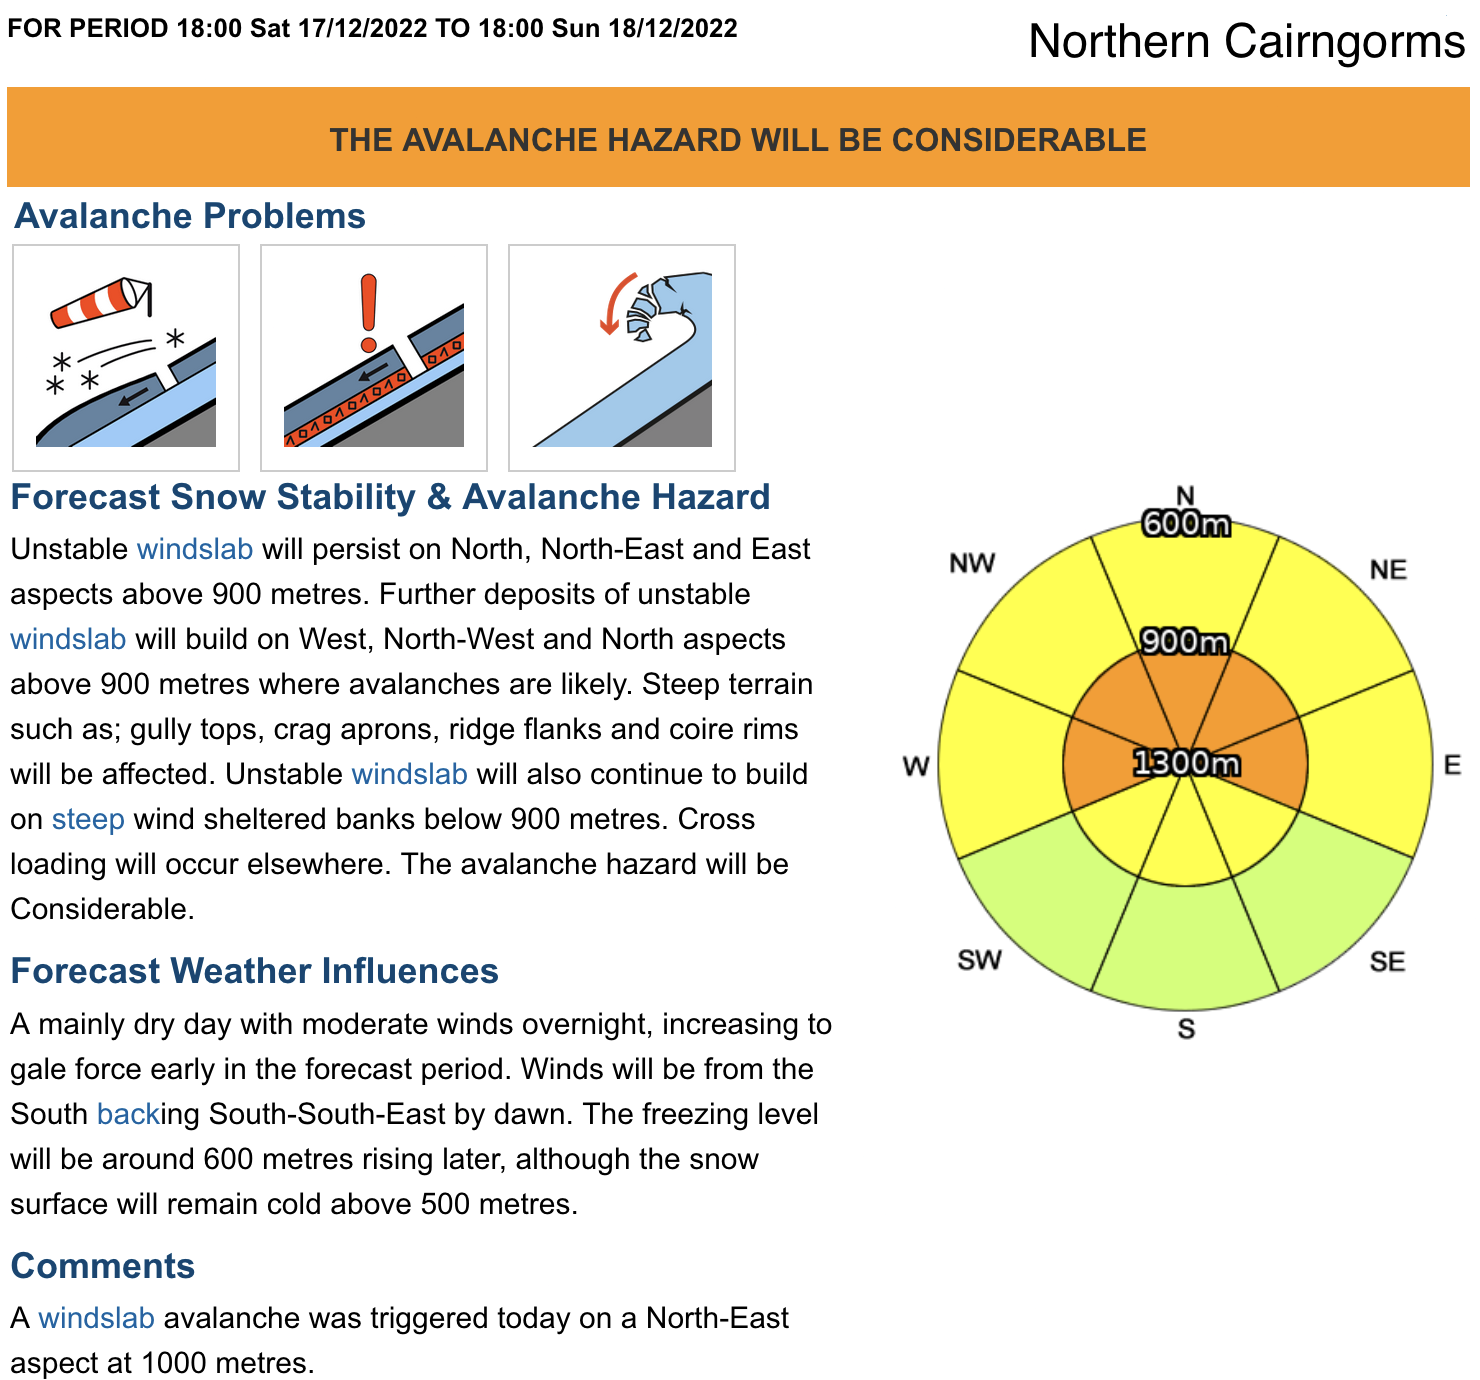
\includegraphics[width=0.90
            \textwidth]{assets/3rdparty/sais_sample_report_adapted.png}}
			\caption{Forecast from www.sais.gov.uk, date matches Figure \ref{fig:sample_prediction}}
		\label{fig:sample_report}
	\end{figure}

\end{block}

\begin{block}{Data}

   % Exactly where did your data come from and what does your contain? (ie. What are in the rows and columns? Are examples labeled with ground truth? If you have images, are they color, normalized, etc?) 
   % (2-3 sentences max)

   The avalanche danger level forecast data used as dependent variable comes from \href{https://www.sais.gov.uk/forecast-archive/}{Scottish Avalanche Information Service} (SAIS), the observed avalanche danger level (published on the date for which forecast was made, after a field trip by avalanche professionals) was used as one of the baselines (see Table \ref{tbl:sais_eval}).
    
	The weather data used for independent variables comes from \href{https://www.visualcrossing.com/}{Visual Crossing} who were kind enough to grant us free access to their data for research purposes.

    The size of the combined dataset after cleansing is 9,831 observations spread across 6 forecast areas ranging from 2007 to 2024 (end of previous season) and split 80/20 into training and test sets (cross-validation was used for hyperparameter tuning).

\end{block}

\end{column}

\separatorcolumn

\begin{column}{\colwidth}

\begin{block}{Features}

    % How many features do you have and which features are the raw input data (ex. color, weight, location, etc) vs. features you have derived (ex. ICA, Gaussian Kernel)? Why they are appropriate for this task? (3-4 sentences max)

    
The weather data for the highest summit in each of the 6 forecast zones has been downloaded from \href{https://www.visualcrossing.com/}{Visual Crossing}. All the standard atmospheric variables like temperature, humidity, precipitation, wind speed and direction have been downloaded along with selected \href{https://www.visualcrossing.com/resources/documentation/weather-api/agriculture-elements-in-the-timeline-weather-api/}{agricultural} and \href{https://www.visualcrossing.com/resources/documentation/weather-api/energy-elements-in-the-timeline-weather-api/}{energy} data points (details can be found in \href{https://github.com/witgaw/avalanche-danger-level-forecast/blob/project-report/src/data-exploration-weather.ipynb}{\texttt{data-exploration-weather.ipynb}} in the open source project repository linked at the bottom).

Since avalanches are impacted by weather not just the day before the warning is issued but over many days prior, we have transformed the data so that our independent variables reflect that by stacking hourly data for the first 48 hours followed by 136 entries of daily data (from the beginning of each season, padding with zeros for dates early in the season) for each feature. \\
After cleaning up the data to remove missing variables the dimensionality of the independent variable vector ended up being 4,554.

	% Since avalanches, and thus avalanche hazard forecasts, are impacted by weather not just the day before the warning is issued but over many days prior, or even the entire season, we have transformed the data so that our independent variables reflect that. For the day for which the hazard level is modelled, as well as the day prior,u we use hourly data for all the variables considered. For all previous days we use daily data. We account for \input{assets/snippets/sais_avg_season_length.txt}days as that's the average season length in our dataset. All the entires prior to season's begining are set to 0. Thus the vectors are sparser the closer to the begining of the season the modelled hazard level is. 

    
\end{block}

  \begin{block}{Models}

   % Exactly which model(s) are you using? Write out the basic math formulas and clearly note any modifications oradditions. If you have more than one model, make subsections for each. (3-4 sentences max)
 All of the models used in this project have been covered in CS224 this term (Fall 2024), for the sake of brevity we refer the reader interested in details and formulations of these models to the lecture notes.
   
 \underline{\textbf{Softmax regression}}\\

	Softmax regression, also known as multinomial logistic regression, is a generalization of logistic regression to multiple classes.
    
    % , where probability that for a given input vector $\mathbf{x}$ the danger level is $l$ is:\\ $P(y = l \mid \mathbf{x}; \theta_l)=\frac{\exp(\theta_l^\top \mathbf{x})}{\sum_{j=1}^4 \exp(\theta_j^\top \mathbf{x})}$ and the level with highest probability is used as the model output.

 \underline{\textbf{Random forest}}\\
	 Random forest is an ensemble learning technique combining multiple decision trees and averaging their results to generate the output which helps to reduce the tendency of decision trees to overfit the data.

 \underline{\textbf{Multi-layer perceptron}}\\
Due to the high dimensionality of the data, highly non-linear relationship between weather data across the entire season and the avalanche danger level, and since we are dealing with a classification problem, a multi-layer neural network seemed like a promising approach to try out for this problem.

  \end{block}

  \begin{block}{Results}

    % Make a compact table of results. Each row should be a different model. The columns should be the training error and the test error. List how many samples are in each of the training and testing data sets. Obviously, these sets should be different. (1-2 sentences max + 1 table max)

    \begin{table}[H]
\caption{Evaluation metrics. MSE = mean squared error, 
const = output level 3 for any input (baseline), obs. = observed hazard level (baseline),
SM = softmax, RF = Random forest, MLP = Multi-layer perceptron, T = tuned}
\label{tbl:sais_eval}
\begin{tabular}{l*{8}{p{2.9cm}}}
\toprule
 & const  & obs.    & SM     & SM(T) & RF    & MLP    & RF(T)  & MLP(T) \\
\midrule
Training set &  &  &  &  &  &  &  &  \\
\midrule
MSE & 1.63 & 0.31  & 0.13 & 0.25 & 0.00 & 0.14 & 0.00 & 0.06 \\
\midrule
Test set &  &  &   &  &  &  &  &  \\
\midrule
MSE & 1.63 & 0.30  & 0.55 & 0.58 & 0.37 & 0.49 & 0.44 & 0.41 \\
average error & -0.89 & 0.15  & 0.01 & -0.08 & 0.04 & -0.00 & 0.03 & 0.03 \\
accuracy & 0.33 & 0.76  & 0.60 & 0.61 & 0.70 & 0.65 & 0.67 & 0.68 \\
precision: &  &  &    &  &  &  &  &  \\
precision (macro-averaged) & 0.08 & 0.74  & 0.57 & 0.56 & 0.73 & 0.64 & 0.72 & 0.66 \\
recall (macro-averaged) & 0.25 & 0.69  & 0.57 & 0.61 & 0.58 & 0.58 & 0.57 & 0.63 \\
$F_1$ (macro-averaged) & 0.12 & 0.70  & 0.57 & 0.57 & 0.60 & 0.60 & 0.59 & 0.64 \\
\bottomrule
\end{tabular}
\end{table}

    
\begin{figure}[htbp]
    \centering
    \begin{subfigure}[b]{0.32\textwidth}
        \centering
        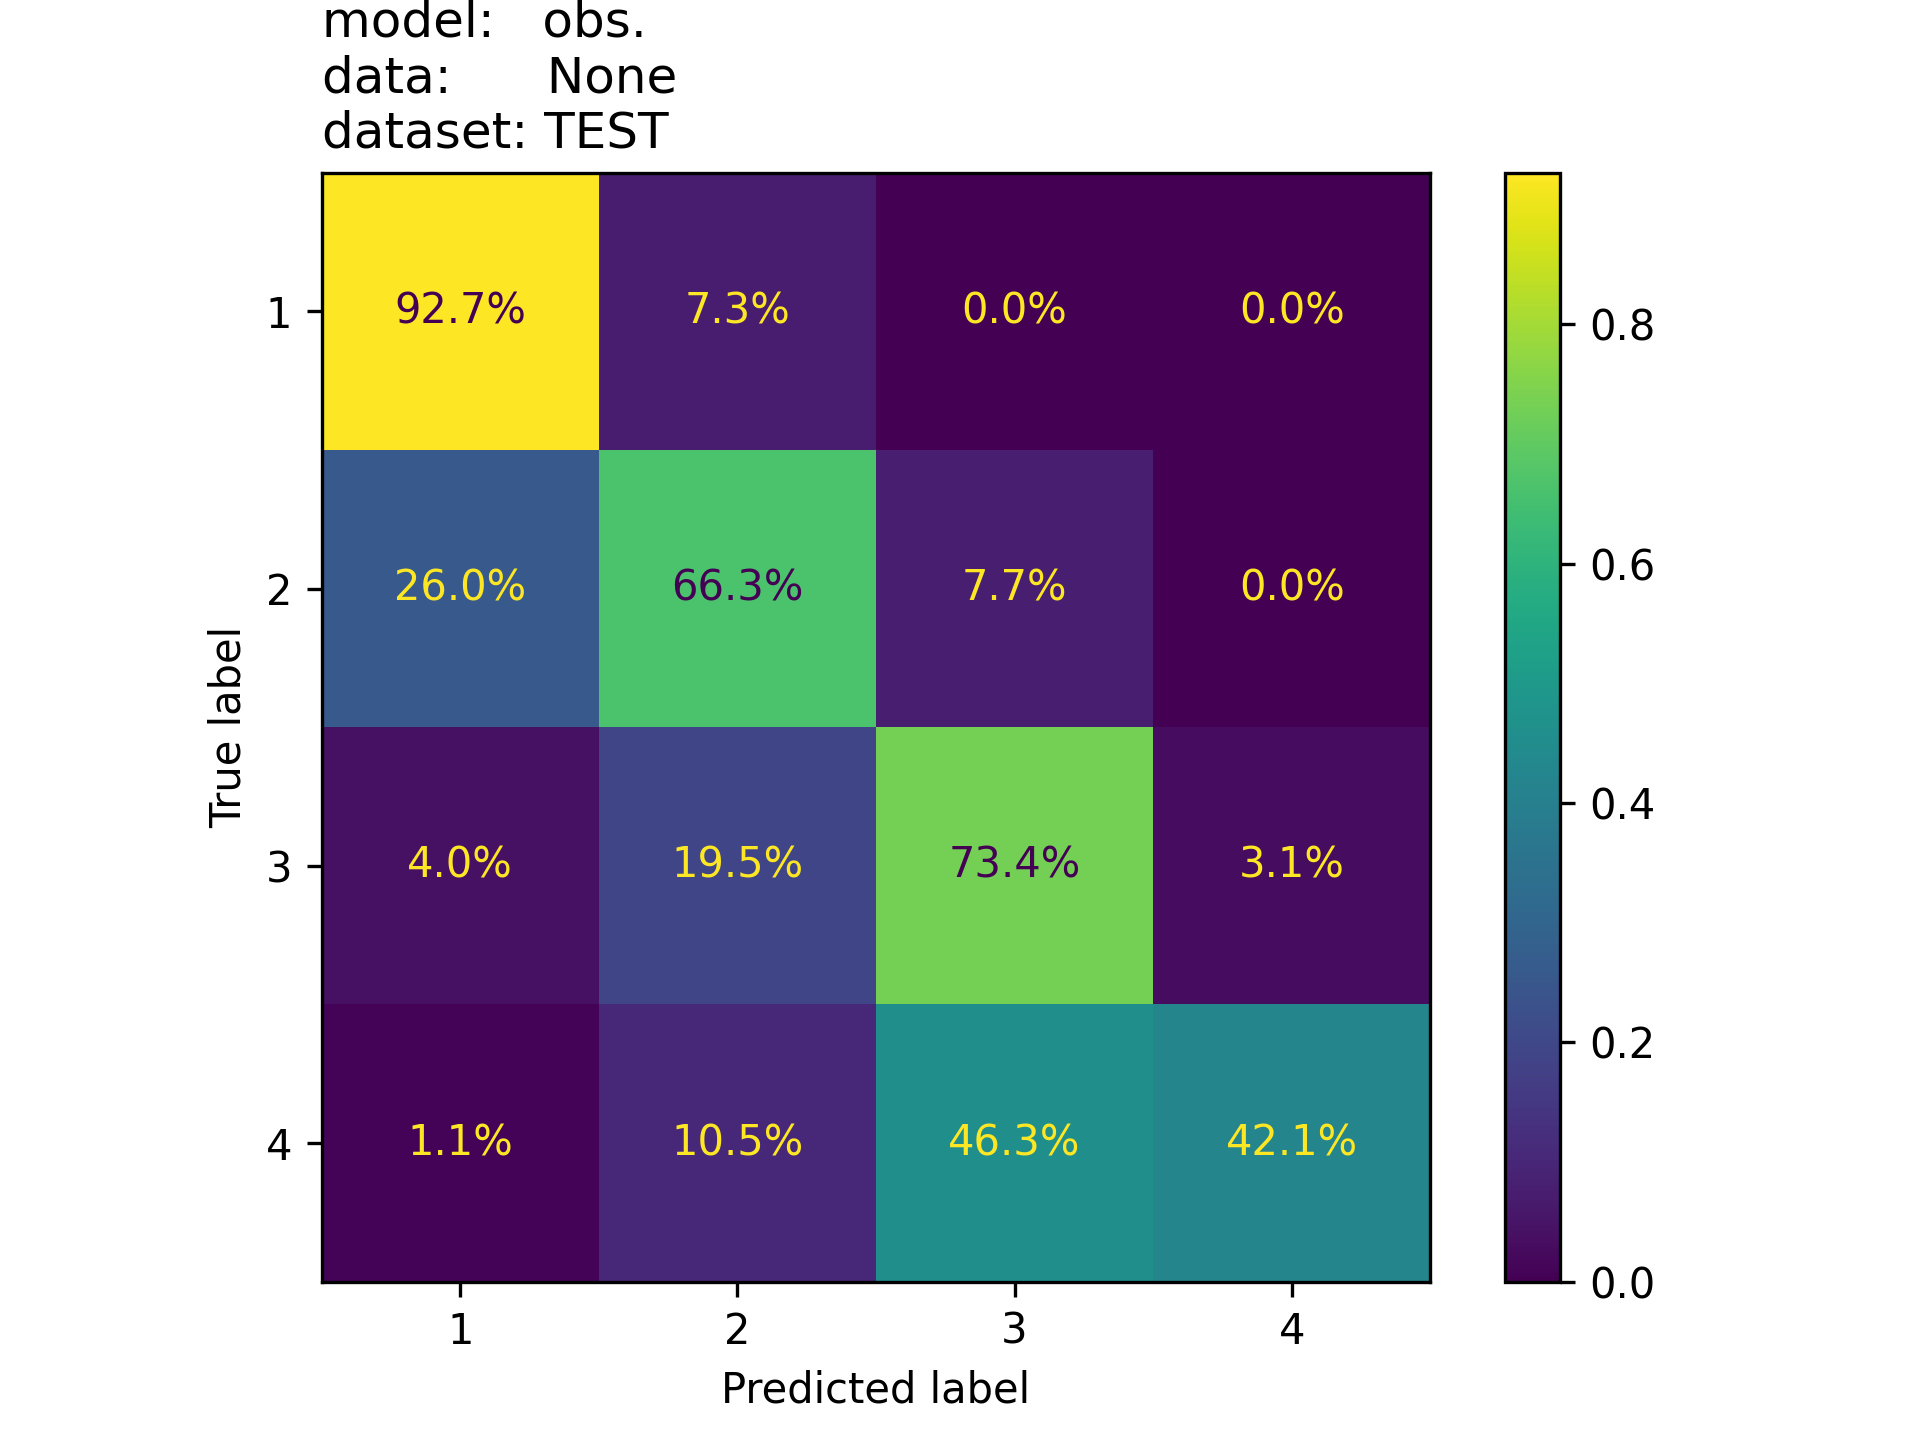
\includegraphics[width=\textwidth]{assets/figures/sais_confusion_matrix_obs.___None_test.png}
        \caption{Observed hazard levels (baseline)}
        \label{fig:subfig1obs}
    \end{subfigure}
    \hfill
    \begin{subfigure}[b]{0.32\textwidth}
        \centering
        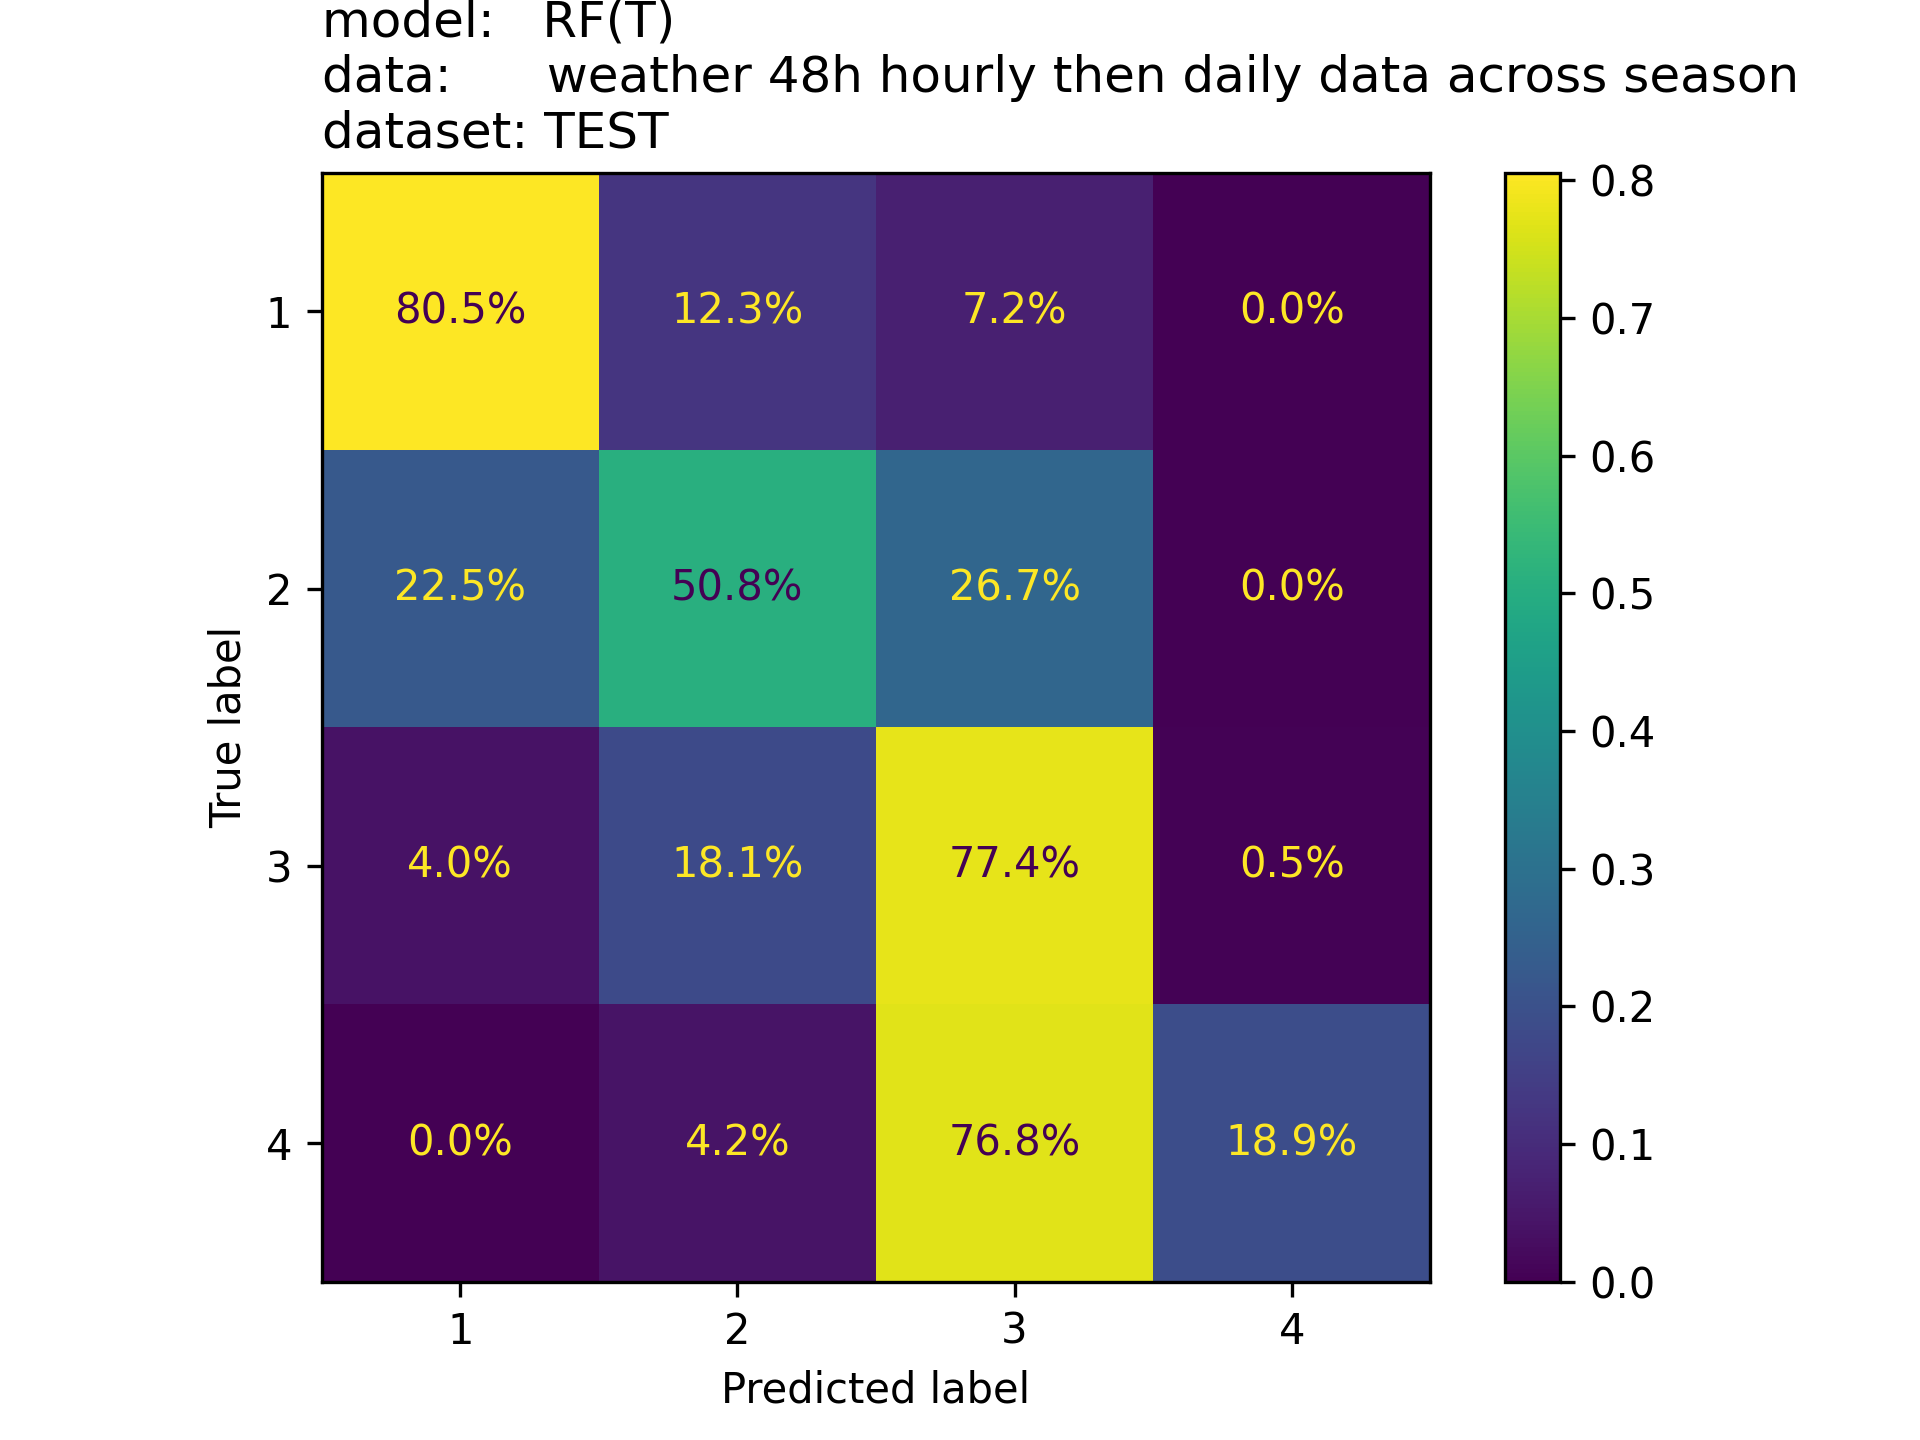
\includegraphics[width=\textwidth]{assets/figures/sais_confusion_matrix_RF(T)__weather_48h_hourly_then_daily_data_across_season_test.png}
        \caption{RF after hyperparameter tuning}
        \label{fig:subfig2rf}
    \end{subfigure}
    \hfill
    \begin{subfigure}[b]{0.32\textwidth}
        \centering
        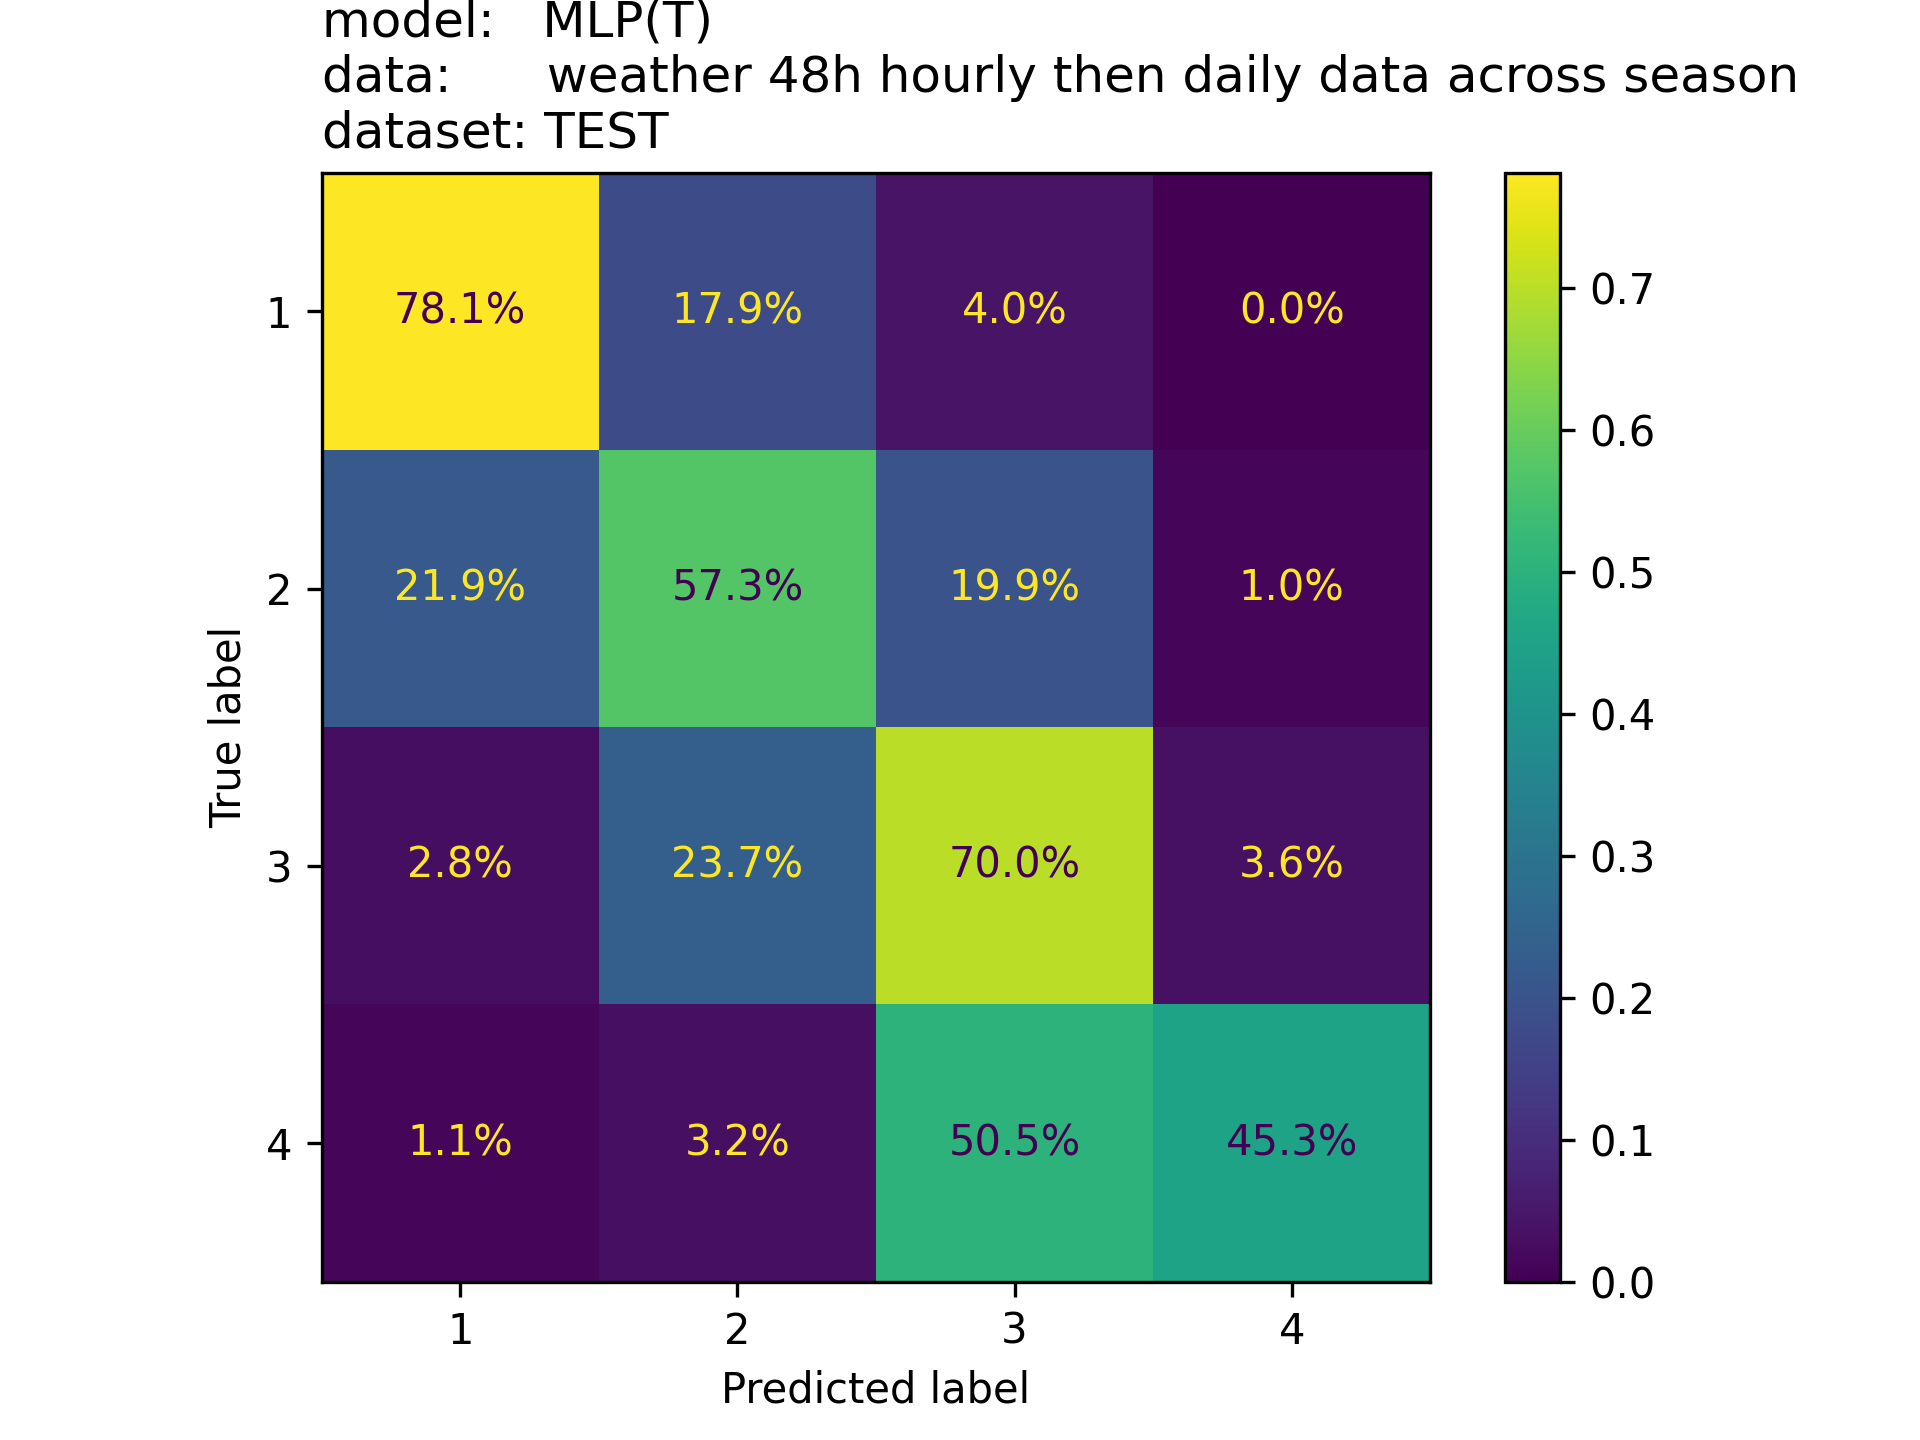
\includegraphics[width=\textwidth]{assets/figures/sais_confusion_matrix_MLP(T)_weather_48h_hourly_then_daily_data_across_season_test.png}
        \caption{MLP after hyperparameter tuning}
        \label{fig:subfig3mlp}
    \end{subfigure}
    \caption{Selected confusion matrices}
    \label{fig:confusion_matrices}
\end{figure}

  \end{block}

\end{column}

\separatorcolumn

\begin{column}{\colwidth}

  \begin{block}{Discussion}

    % This is where you share your thoughts about your project. (Hopefully you have a few interesting interpretations!) Brieflysummarized what just happened. Briefly explain whether or not you expected your results. If your results were good, explain why. If they were not good, explain why. (6 sentences max)

	The multi-layer perceptron classifier (Figure \ref{fig:subfig3mlp}) is the most promising of the classifiers considered. 
    
	In fact it's not miles away from results presented in \cite{egusphere-2024-2374} which shows performance of a random forest classifier used operationally (for several seasons now) as one of the decision inputs to avalanche danger level forecasts in Swiss alps. 

    Both the paper referenced above and plots in Figure \ref{fig:confusion_matrices} show that while accurately predicting hazard levels  "1" and "3" is quite an attainable goal, most models struggle more with levels "2" and "4". 

    The reason for poor predictive power for level "4" is likely that it's quite rare for that level to be announced by avalanche services (in our dataset it's less that 5\%). On the other hand, the relative frequency of levels "1" to "3" is almost the same across these levels in our dataset. It may be that differences between level "2" and its neighbouring levels are more subtle and not easily identifiable from weather forecast alone, but have more to do with the specifics of a given forecast area.

\begin{figure}[htbp]
    \centering
        \centering
        \frame{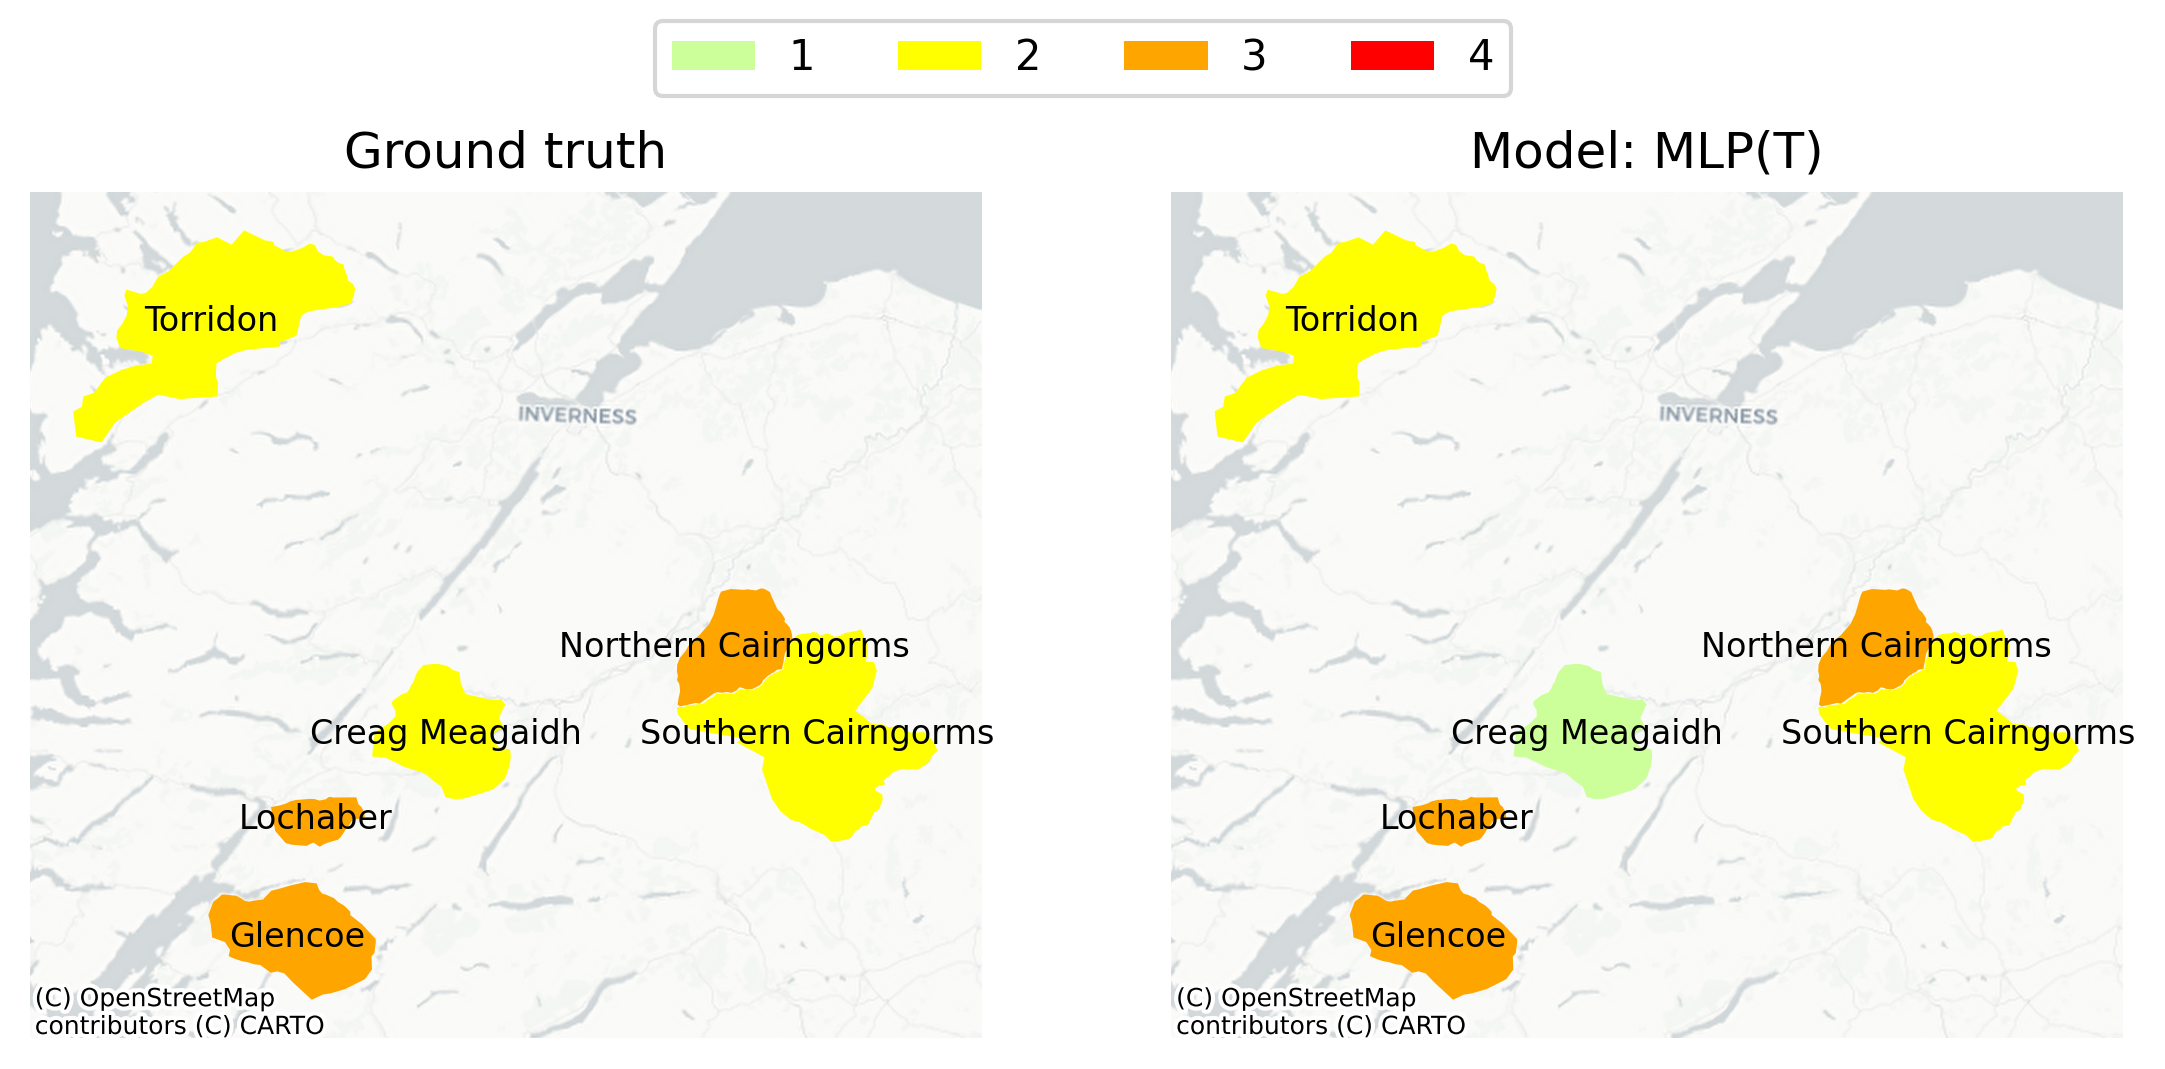
\includegraphics[width=\textwidth]{assets/figures/forecast_plot_MLP(T)_2022-12-17.png}}
    \caption{Ground Truth vs MLP(T) model predictions for a randomly selected date from the test set (17/12/2022).}
    \label{fig:sample_prediction}
\end{figure}
    
  \end{block}

  \begin{block}{Future}

    % If you had another 6 months to work on this, what would you do first? (2-3 sentences max)

	As can be seen in Figure \ref{fig:sample_report}, avalanche reports often contain much more information than just the avalanche hazard levels. Incorporating terrain features to allow for generation of the aspect-elevation rose as well as better generalisation of the model to areas it has not been trained on will be one of the future goals for this project, as well as predicting the type of the avalanche problem from data.

    Since the results obtained with MLP were the most promising, another avenue worth exploring seems to be moving to a more Deep Learning-oriented library like \texttt{PyTorch} or \texttt{TensorFlow} (this project used \texttt{scikit-learn}) and exploring multilayer neural networks with more complex topologies there.

  \end{block}

  \begin{block}{References}

    \nocite{*}
    % \scalebox{0.8}{\bibliographystyle{plain}\bibliography{references}}
    \tiny{\bibliographystyle{plain}\bibliography{references}}

  \end{block}

\end{column}

\separatorcolumn
\end{columns}
\end{frame}

\end{document}
